%!TeX root = main.tex
\chapter{DIE Klasse der Fourier-Transformationen}
In diesem Kapitel werden Beispiele einer speziellen Klasse von $\cD$-Moduln
diskutiert. Dazu wird im folgendem zu 2 Beispielen unter anderem explizit der
Beweis aus \cite{sabbah_cimpa90} zur Levelt-Turrittin-Zerlegung nachvollzogen.

Es wird zunächst ein allgemeines Rezept gegeben, welches zu gegebenem $\phi$
D-Moduln ergibt. Im laufe des Kapitels werden immer speziellere $\phi$
betrachtet und zuletzt wird für konkrete Beispiele eine explizite Rechnung
gegeben.

\section{Rezept für allgemeine $\phi$} \label{sec:allgemeinProblem}
Hier wollen wir nun eine Spezielle Klasse von Meromorphen Zusammenhängen, die
die durch das folgende Rezept entstehen.
\begin{enumerate}
\item Wähle zunächst ein $\phi$
$\in\{\phi=\sum_{k\in I}\frac{a_k}{t^{k}}|I\subset\N\mbox{ endlich}
,a_k\in \C\}$
aus
\item und beginne mit $\sE^{\phi}$. Es gilt
\begin{align*}
\sE^{\phi} &= \cD_{\hat L}/\cD_{\hat L}\cdot (\partial_t-\frac{d}{dt}\phi(t))
\\&=\cD_{\hat L}/\cD_{\hat L}\cdot (\underset{\in\C[t]\subset\cD_{\hat L}^*}
    {\underbrace{\mbox{Hauptnenner }}}
  \cdot (\partial_t-\frac{d}{dt}\phi(t)))
\\&=\cD_{\hat L}/\cD_{\hat L}\cdot ( \underset{=:Q(t,\partial_t)}{\underbrace{
  t^{\max(I)+1} \cdot (\partial_t-\frac{d}{dt}\phi(t))}})
\end{align*}
\begin{comment}
Dies ändert den Meromorphen Zusammenhang nicht, weil $t^{\max(I)+1}$ eine
Einheit in $\cD_{\hat L}$ (und auch in $\cD_{L}$) ist.
\end{comment}
\item Fouriertransformiere $\sE^{\phi}$ und erhalte
\begin{align*}
\,^\cF\!\sE^{\phi}&=\cD_{\hat L}/\cD_{\hat L}\cdot{\cF_Q(z,\partial_z)}
\\&\bydef \cD_{\hat L}/\cD_{\hat L}\cdot 
  \underset{\in\C[z]<\partial_z>}{\underbrace{Q(\partial_z,-z)}}
\end{align*}
\item Betrachte den Zusammenhang bei Unendlich, also wende den Übergang
$x\rightsquigarrow z^{-1}$ an.\\
Was passiert mit der Ableitung $\partial_x$?
Es gilt
\[
\partial_x (f(\frac{1}{x}))=
\partial_z(f)\cdot (-\frac{1}{x^2})=
-\partial_z(f)\cdot z^2= %TODO: wegen klammerung?
- z^2 \cdot \partial_z(f)
\]
also $ \partial_x\rightsquigarrow-z^2\partial_z $.
\[
P_\phi(x,\partial_x):=\cF_Q(x^{-1},-x^2\partial_x) \in \C[t]<\partial_t>
\]
\end{enumerate}
Im folgendem werden wir den zum Minimalpolynom $P_\phi$ assoziierten
Meromorphen Zusammenhang $\cM_\phi=\cD_{\hat K}/\cD_{\hat K}\cdot P_{\phi}$
betrachten.

Wen wir ein spezielles $\phi=\sum_{k\in I}\frac{a_k}{t^{k}}$ betrachten, können
wir das entstehende $P_\phi$, wie folgt, explizit berechnen
\begin{align*}
Q(t,\partial_t) &= t^{\max(I)+1}(\partial_t-\frac{d}{dt}\phi(t))
\\&=t^{\max(I)+1}\Big(\underset{\in \C[t][t^{-1}]<\partial_t>}{\underbrace{
    \partial_t+\sum_{k\in I} k\frac{a_k}{t^{k+1}}}}\Big)
\\&=t^{\max(I)+1}\partial_t 
  + \sum_{k\in I} k\underbracket{\frac{a_k}{t^{k-\max(I)}}}
\\&=t^{\max(I)+1}\partial_t +\sum_{k\in I}k \overbracket{a_k t^{\max(I)-k}}
  & \in \C[t]<\partial_t>
\\\cF_Q(z,\partial_z) &=Q(\partial_z,-z)
\\&=-\partial_z^{\max(I)+1}z +\sum_{k\in I}k a_k\partial_z^{\max(I)-k}
\end{align*}
und damit ist
\begin{align*}
P_{\phi}(x,\partial_x) &=\cF_Q(x^{-1},-x^2\partial_x)
\\&=\underbracket{-(-x^2\partial_x)^{\max(I)+1}x^{-1}}
  +\sum_{k\in I}k a_k(-x^2\partial_x)^{\max(I)-k}
\\&=\overbracket{(-x^2\partial_x)^{\max(I)} x^2\underbracket{\partial_xx^{-1}}}
   +\sum_{k\in I}k a_k(-x^2\partial_x)^{\max(I)-k}
\\&=(-x^2\partial_x)^{\max(I)}
   \underbracket{ x^2 \overbracket{(x^{-1}\partial_x-x^{-2})} }
   +\sum_{k\in I}k a_k(-x^2\partial_x)^{\max(I)-k}
\\&=(-x^2\partial_x)^{\max(I)} \overbracket{(x\partial_x-1)}
   +\sum_{k\in I}k a_k(-x^2\partial_x)^{\max(I)-k}
  & \in \C[x]<\partial_x>
\end{align*}
Im Anhang \ref{chap:zu-rezept} wird das $(x^2\partial_x)^{k}$ genauer
diskutiert. Dies führt aber hier an dieser Stelle nicht mehr weiter in die
gewünschte Richtung.

\paragraph{Ab jetzt nur noch für den Spezialfall $\phi=\frac{a}{t^{q}}$.}
Also sei $\cM_\phi=\cD_{\hat K}/\cD_{\hat K}\cdot P_\phi$ mit
\[
P_{\phi}(x,\partial_x) =(-x^2\partial_x)^{q} (x\partial_x-1)+qa \,,
\]
so dass
\begin{lem}
Es gilt $\cP(\cM_{\phi})=\{\frac{q}{q+1}\}$.
\end{lem}
\begin{comment}
\begin{lem}
$N((x^2\partial_x)^q)=N(x^{2q}\partial_x^q)$
\end{lem}
\end{comment}
\begin{proof} \cite[5.b.]{sabbah_Fourier-local}
Um zu zeigen, dass die Behauptung gilt, formen wir $P_{\phi}$ um und isolieren
die Monome, die für das Newton-Polygon von bedeutung sind.
\begin{align*}
N\Big(P_{\phi}(x,\partial_x)\Big) &= N\Big(\underbracket{(-x^2\partial_x)^{q}}
  (x\partial_x-1)+qa\Big)
\\&= N\Big(\overbracket{\underset{\text{liefert keinen
Beitrag}}{\underbrace{(-1)^q}}(x^{2q}\partial_x^q 
  + \underset{\text{liefern keinen Beitrag}}{\underbrace{\textbf{T.h.O.}}}}) 
  (x\partial_x - 1) + qa \Big)
\\&= N\Big( \underbracket{x^{2q}\partial_x^q (x\partial_x - 1)} + qa \Big)
\\&= N\Big(\overbracket{x^{2q}\underbracket{\partial_x^q x}\partial_x
  - x^{2q}\partial_x^q} + qa \Big)
\\&= N\Big(x^{2q}\overbracket{(x\partial_x^q + q\partial_x^{q-1})}\partial_x
  - x^{2q}\partial_x^q + qa \Big)
\\&= N\Big(x^{2q + 1}\partial_x^{q + 1} 
  + \underset{\text{liefern keinen Beitrag}}{
  \underbrace{qx^{2q}\partial_x^{q} - x^{2q}\partial_x^q}} + qa \Big)
\\&= N\Big(x^{2q + 1}\partial_x^{q + 1} + qa \Big)
\end{align*}
\begin{comment}
ist vlt besser \emph{Therme niedriger Ordnung} zu verwenden??
\end{comment}
Wobei hier das \textbf{T.h.O} eine Abkürzung für \emph{Therme höherer Ordnung}
ist. Hier ist ein Term $\epsilon x^{p}\partial_x^{q}$, mit $\epsilon\in \C, p,q
\in \Z$, von höherer Ordnung als
$\tilde\epsilon x^{\tilde p}\partial_x^{\tilde q}$, mit $\tilde\epsilon\in \C,
\tilde p,\tilde q \in \Z$, falls $q>\tilde q$ und $p-q<\tilde p - \tilde q$.
Anschaulich bedeutet das, dass 
\[
\Big( (q,p-q) + \R_{\leq 0} \times \R_{\geq 0} \Big) \supset 
\Big( (\tilde q,\tilde p-\tilde q) + \R_{\leq 0} \times \R_{\geq 0} \Big) \,.
\]
Offensichtlich ist damit $ N(\epsilon x^{p}\partial_x^{q}+\tilde\epsilon
x^{\tilde p}\partial_x^{\tilde q}) =N(\epsilon x^{p}\partial_x^{q}) $, also
können Therme höherer Ordnung vernachlässigt werden, wenn das
Newton-Polygon gesucht ist.
\begin{figure}[H]
\caption{Newton Polygon zu $P_{\phi}$}
\begin{center}
\fbox{
  \begin{tikzpicture}[scale=.7,descr/.style={fill=white,inner sep=2.5pt}]
  \def\myPoints{0/0,6/5}
  \def\myPath{ -- node[descr]{$\frac{q}{q+1}$} (6,5)}
  \myPlotFunction{\myPoints}{\myPath}{6}{0}{5}{$(q+1,q)$}
  \end{tikzpicture}
}
\end{center}
\end{figure}
\begin{comment}
TODO: ist T.h.O. hier die richtige formulierung?? besser:
\begin{align*}
N\Big(P_{\phi}(x,\partial_x)\Big) &= N\Big(\underbracket{(-x^2\partial_x)^{q}}
  (x\partial_x-1)+qa\Big)
\\&= N\Big(\overbracket{\underset{\text{liefert keinen
Beitrag}}{\underbrace{(-1)^q}}(x^{2q}\partial_x^q 
  + \underset{\text{liefern keinen Beitrag, weil $\mu_i(x)\in x^{q+i}\Cfx$}}{
  \underbrace{
  \mu_{q-1}(x)\partial_x^{q-1} + \dots + \mu_{1}(x)\partial_x + \mu_0(x)}}
  )}
  (x\partial_x - 1) + qa \Big)
\\&= N\Big(x^{2q}\partial_x^q
  (x\partial_x - 1) + qa \Big)
\\&= N\Big(x^{2q}\underbracket{\partial_x^q x}\partial_x
  - x^{2q}\partial_x^q + qa \Big)
\\&= N\Big(x^{2q}\overbracket{(x\partial_x^q + q\partial_x^{q-1})}\partial_x
  - x^{2q}\partial_x^q + qa \Big)
\\&= N\Big(x^{2q + 1}\partial_x^{q + 1} 
  + \underset{\text{liefern keinen Beitrag}}{
  \underbrace{qx^{2q}\partial_x^{q} - x^{2q}\partial_x^q}} + qa \Big)
\\&= N\Big(x^{2q + 1}\partial_x^{q + 1} + qa \Big)
\end{align*}
\end{comment}
\end{proof}
Also ist ein pull-back mit Grad $q+1$ nötig, um einen ganzzahligen Slope zu
bekommen.
Sei $\rho:t\mapsto x:=-(q+1) t^{q+1}$ so ist
\begin{align*}
\rho^+\cM_\phi &= \rho^+(\cD_{\hat K}/\cD_{\hat K}\cdot P_\phi(x,\partial_x))\\
  &=\cD_{\hat K}/\cD_{\hat K}\cdot(\rho^*P_\phi(x,\partial_x))\\
  &=\cD_{\hat K}/\cD_{\hat K}\cdot(P_\phi(\rho(t),\rho'(t)^{-1}\partial_t))\\
  &=\cD_{\hat K}/\cD_{\hat K}
    \cdot(P_\phi(-(q+1) t^{q+1},-\frac{1}{(q+1)^2t^q}\partial_t))\\
  &=\cD_{\hat K}/\cD_{\hat K} \cdot
    ((\underbracket{-(-(q+1) t^{q+1})^2\frac{-1}{(q+1)^2t^{q}}\partial_t})^{q}
    (\underbracket{-(q+1) t^{q+1}\frac{-1}{(q+1)^2t^{q}}\partial_t}-1)+qa)\\
  &=\cD_{\hat K}/\cD_{\hat K}
    \cdot((\overbracket{
      \underbracket{-\frac{-(q+1)^2}{(q+1)^2}t^{2(q+1)-q}}\partial_t})^{q}
    (\overbracket{\frac{1}{q+1}t\partial_t}-1)+qa)\\
  &=\cD_{\hat K}/\cD_{\hat K}
    \cdot((\overbracket{t^{q+2}}\partial_t)^{q}
    (\frac{1}{q+1}t\partial_t-1)+qa)\\
  &=\cD_{\hat K}/\cD_{\hat K}
    \cdot((t^{q+2}\partial_t)^{q}
    (t\partial_t-(q+1))+(q+1)qa)
\end{align*}
\begin{comment}
muss noch gezeigt werden, dass dies ein Meromorpher Zusammenhang???
\end{comment}
\begin{comment}
Bei \cite{sabbah_Fourier-local}:\\
Sei $\rho:t\mapsto x:=-\frac{t^{q+1}}{qa}$ so ist
\begin{align*}
\rho^+\cM_\phi &= \rho^+(\cD_{\hat K}/\cD_{\hat K}\cdot P_\phi(x,\partial_x))\\
  &=\cD_{\hat K}/\cD_{\hat K}\cdot(\rho^*P_\phi(x,\partial_x))\\
  &=\cD_{\hat K}/\cD_{\hat K}\cdot(P_\phi(\rho(t),\rho'(t)^{-1}\partial_t))\\
  &=\cD_{\hat K}/\cD_{\hat K}
    \cdot(P_\phi(-\frac{t^{q+1}}{qa}, -\frac{qa}{(q+1)t^q}\partial_t))
\end{align*}
mit
\begin{align*}
P_\phi(-\frac{t^{q+1}}{qa}, -\frac{qa}{(q+1)t^q}\partial_t)
  &= (-(-\frac{t^{q+1}}{qa})^2(-\frac{qa}{(q+1)t^q}\partial_t))^q
    (-\frac{t^{q+1}}{qa}(-\frac{qa}{(q+1)t^q}\partial_t)-1)+qa\\
  &= ((\frac{t^{q+1}}{qa})^2\frac{qa}{(q+1)t^q}\partial_t)^q
    (\frac{t^{q+1}}{qa}\frac{qa}{(q+1)t^q}\partial_t-1)+qa\\
  &= (\frac{(t^{q+1})^2}{qa(q+1)t^q}\partial_t)^q
    (\frac{t^{q+1}}{(q+1)t^q}\partial_t-1)+qa\\
  &= (\frac{t^{2q+2-q}}{qa(q+1)}\partial_t)^q
    (\frac{t^{q+1-q}}{(q+1)}\partial_t-1)+qa\\
  &= (\frac{t^{q+2}}{qa(q+1)}\partial_t)^q
    (\frac{1}{(q+1)}t\partial_t-1)+qa\\
\end{align*}
\end{comment}
mit $\cP(\rho^+\cM_\phi)=\{q\}\subset\N$. Definiere mittels
$q=\frac{q}{1}=:\frac{\lambda_0}{\lambda_1}$ die  Linearform
\[
L(s_0,s_1)=\lambda_0s_0+\lambda_1s_1=qs_0+s_1 \,.
\]
Schreibe $\rho^*P_{\phi}=\sum_i\sum_j\alpha_{ij}t^j\partial_t^i$ und berechne
die \emph{Determinanten Gleichung} $\sigma_L(\rho^*P_{\phi})\in \hat L[\xi]$.
\begin{comment}
Schon gezeigt, das $ord_L = 0$?
\end{comment}
\begin{align*}
\sigma_L(\rho^*P_{\phi})
  &= \sum_{\{(i,j)\in\N\times\Z \mid L(i,i-j)=0\}}\alpha_{ij}t^j\xi^i\\
  &= \sum_{\{(i,j)\in\N\times\Z \mid (q+1)i-j=0\}}\alpha_{ij}t^j\xi^i
\end{align*}
Da $\hat L[\xi]$ kommutativ ist gilt hier, dass $(t^j\xi^i)^k=t^{jk}\xi^{ik}$ ist.
Setze $\theta=t^{\lambda_0+\lambda_1}\xi^{\lambda_1}=t^{q+1}\xi$ so können wir
\begin{align*}
\sigma_L(\rho^*P_{\phi}) &= \sum_{k\geq 0}\alpha_k\theta^k & & \alpha_k\in\C
\end{align*}
schreiben, welches wir als nächsten Schritt faktorisieren
\[
\sigma_L(\rho^*P_\phi)=\epsilon\prod_{\beta}(\theta-\beta)^{\gamma_\beta}\,.
\]
Wobei $\epsilon\in\C^\times$ eine Konstante ist.
Sei $\beta_0$  eine der Nullstellen.
Da $\ord_L(\rho^*P_\phi)=0$ und der einzige Slope von $\rho^*P_\phi$ nicht
gleich $0$ ist, gilt offensichtlich, dass $\alpha_0\neq0$. Also ist $0$ keine
Nullstelle von $\sigma_L(\rho^*P_\phi)$.
Setze $\psi(x):=(\beta_0/\lambda_0)t^{-\lambda_0}=(\beta_0/q)t^{-q}$ und
betrachte
\begin{align*}
\cN:=\rho^+\cM_\phi\otimes\sE_{\hat L}^\psi
  &= \cD_{\hat L}/\cD_{\hat L}\cdot(\rho^*P_{\phi})\otimes\sE_{\hat L}^\psi \,.
\end{align*}
\begin{lem}
Sei $e$ ein zyklischer Vektor zu $\rho^+\cM_\phi$, so ist $e\otimes
\underset{\in\hat L}{\underbrace{1}}\in\cN$ ein zyklischer Vektor für
$\cN\bydef\rho^+\cM_\phi\otimes\sE_{\hat L}^\psi$.
\end{lem}
\begin{proof}
Es sei $e$ ein zyklischer Vektor von $\rho^+\cM_{\phi_1}$.
Da der Grad von $\rho^*P_{\phi}$ gleich $q+1$ ist, ist auch die Dimension von
$\rho^+\cM$ gleich $q+1$. Damit ist auch $\dim_K\cN=q+1$, also reicht zu
zeigen, dass $e\otimes 1$, $\partial_t(e\otimes 1)$, $\partial_t^2(e\otimes
1)$, ,\dots, $\partial_t^{q}(e\otimes 1)$ ein linear unabhängiges System ist.
Es gilt
\begin{align*}
\partial_t(e\otimes 1) &= (\partial_t e)\otimes 1 + t\otimes \partial_t 1\\
  &= (\partial_t e)\otimes 1 + e\otimes \psi'(t)\\
  &= (\partial_t e)\otimes 1 +  \psi'(t)(e\otimes 1)\\
\partial_t^2(e\otimes 1) &= \partial_t((\partial_t e)\otimes 1 +
    \psi'(t)(e\otimes 1))\\
  &= (\partial_t^2 e)\otimes 1 + (\partial_t e)\otimes \psi'(t)
  + \psi''(t)(e\otimes 1)
  + \psi'(t)((\partial_t e)\otimes 1 + e\otimes \psi'(t))\\
  &= (\partial_t^2 e)\otimes 1
  + \psi'(t)(\partial_t e)\otimes 1
  + \psi''(t)(e\otimes 1)
  + \psi'(t)(\partial_t e)\otimes 1
  + \psi'(t)^2(e\otimes 1)\\
  &= (\partial_t^2 e)\otimes 1
  + 2\psi'(t)(\partial_t e)\otimes 1
  + (\psi''(t) + \psi'(t)^2)(e\otimes 1)\\
  &~\vdots\\
\partial_t^{q}(e\otimes 1) &= (\partial_t^q e)\otimes 1
  + \lambda_{q-1}(\partial_t^{q-1} e)\otimes 1
  +\dots
  + \lambda_{1}(\partial_t e)\otimes 1
  + \lambda_0(e\otimes 1)\\
\end{align*}
und somit ist dann
\[
\begin{pmatrix}
e\otimes 1\\
\partial_t(e\otimes 1)\\
\partial_t^2(e\otimes 1)\\
\vdots\\
\partial_t^{q-1}(e\otimes 1)\\
\partial_t^{q}(e\otimes 1)\\
\end{pmatrix}
=
\begin{pmatrix}
1         & 0         & \cdots & \cdots & \cdots        & 0 \\
\psi'(t)  & 1         & 0      &        &               & \vdots\\
\star     & \star     & 1      & 0      &               & \vdots\\
\vdots    &           & \ddots & \ddots & \ddots        & \vdots\\
\star     & \cdots    & \cdots & \star  & 1             & 0\\
\lambda_0 & \lambda_1 & \cdots & \cdots & \lambda_{q-1} & 1\\
\end{pmatrix}
\begin{pmatrix}
e\otimes 1\\
(\partial_t e)\otimes 1\\
(\partial_t^{2}e)\otimes 1\\
\vdots\\
(\partial_t^{q-1}e)\otimes 1\\
(\partial_t^{q}e)\otimes 1\\
\end{pmatrix}
\]
Da bekanntlich $e\otimes1$, $(\partial_t e)\otimes 1$, $(\partial_t^{2}e)\otimes
1$,\dots, $(\partial_t^{q}e)\otimes 1$ linear unabhängig sind, gilt dies auch
für $e\otimes 1$, $\partial_t(e\otimes 1)$, $\partial_t^2(e\otimes 1)$, ,\dots,
$\partial_t^{q}(e\otimes 1)$. Damit folgt die Behauptung.
\end{proof}
\begin{comment}
\begin{lem}
\cite[Seite 44]{DiplHedwig}
Wenn $\rho^+\cM_\phi=\cD_{\hat K}/\cD_{\hat
K}\cdot(\rho^*P_{\phi}(x,\partial_x))$ gilt, so ist
\begin{align*}
\cN\bydef\rho^+\cM_\phi\otimes\sE_{\hat K}^\psi
  &=\cD_{\hat K}/\cD_{\hat
    K}\cdot(\rho^*P_{\phi}(x,\partial_x+\frac{\beta}{x^{\lambda+1}}))\\
  &=\cD_{\hat K}/\cD_{\hat
    K}\cdot(\rho^*P_{\phi}(x,\partial_x+\frac{\beta}{x^{\lambda+1}}))
\end{align*}
\end{lem}
\end{comment}
Zerlege nun $\cN=\bigoplus_i\cN_i$ wobei $\cN_i$ Meromorphe Zusammenhänge mit
genau einem Slope.
\begin{comment}
TODO: Quelle / Lemma
\end{comment}
Wende auf die $\cN_i$ jeweils die Induktion an und erhalte zu jedem (nach
eventuellem pull-back) eine Zerlegung in reguläre Meromorphe Zusammenhänge.
Nach dem diese mittels $\sE^{-\psi}_{\hat L}$ zurückgetwistet wurden, sind
diese immer noch regulär, aber die direkte Summe davon ist isomorph zu
$\rho^+\cM_{\phi}$.

\section{Spezialfall $\phi_1:=\frac{a}{x}$}
Als konkreten Fall betrachten wir nun $\cM_{\phi_1}$ bezüglich
$\phi_1:=\frac{a}{x}$. Es ist das Minimalpolynom gegeben durch
\begin{align*}
P_{\phi_1}(x,\partial_x) &=-x^2\partial_x (x\partial_x-1)+a
\\&=-x^2\underbracket{\partial_xx}\partial_x+x^2\partial_x+a
\\&=\underbracket{-x^2\overbracket{(x\partial_x+1)}\partial_x} + x^2\partial_x
  + a
\\&=\overbracket{-x^3\partial_x^2 - x^2\partial_x}+x^2\partial_x+a
\\&=-x^3\partial_x^2+a
\end{align*}
Erhalte nun das Newton-Polygon mit den Slopes
$\cP(\cM_{\phi_1})=\{\frac{1}{2}\}$.
\begin{figure}[H]
\caption{Newton Polygon zu $P_{\phi_1}$}
\begin{center}
\fbox{
  \begin{tikzpicture}[scale=1.5,descr/.style={fill=white,inner sep=2.5pt}]
  \def\myPoints{0/0,2/1}
  \def\myPath{ -- node[descr]{$\frac{1}{2}$} (2,1)}
  \myPlotFunction{\myPoints}{\myPath}{2}{0}{1}{$N(P_{\phi_1})$}
  \end{tikzpicture}
}
\end{center}
\end{figure}
Berechne nun zu $\rho:t\mapsto x:=-2t^2$ ein Minimalpolynom $\rho^*P_{\phi_1}$
zu $\rho^+\cM_{\phi_1}$:
\begin{align*}
\rho^*P_{\phi_1}(x,\partial_x)
  &=t^{3}\partial_t(t\partial_t-2)+2a\\
  &=t^{3}\underbracket{\partial_tt}\partial_t-2t^{3}\partial_t+2a\\
  &=t^{3}\overbracket{(t\partial_t+1)}\partial_t-2t^{3}\partial_t+2a\\
  &=t^{4}\partial_t^2+t^{3}\partial_t-2t^{3}\partial_t+2a\\
  &=t^{4}\partial_t^2-t^{3}\partial_t+2a
\end{align*}
\iffalse
  \begin{comment}
  \begin{align*}
  \rho^*P_{\phi_1}(x,\partial_x)
    &=-\frac{1}{2}t^{3}\partial_t
      (\frac{1}{2}t\partial_t-1)+a\\
    &=-\frac{1}{4}t^{3}\underbracket{\partial_tt}\partial_t
      +\frac{1}{2}t^{3}\partial_t+a\\
    &=-\frac{1}{4}t^{3}\overbracket{(t\partial_t+1)}\partial_t
      +\frac{1}{2}t^{3}\partial_t+a\\
    &=-\frac{1}{4}t^{4}\partial_t^2
      \underbracket{-\frac{1}{4}t^{3}\partial_t+\frac{1}{2}t^{3}\partial_t}+a\\
    &=-\frac{1}{4}t^{4}\partial_t^2
      \overbracket{+\frac{1}{4}t^{3}\partial_t}+a
  \end{align*}
  \end{comment}
\fi
und erhalte einen Meromorphen Zusammenhang $\rho^+\cM_{\phi_1}=\cD_{\hat
K}/\cD_{\hat K}\cdot\rho^*P_{\phi_1}$ mit genau dem Slope
$1=\frac{1}{1}=:\frac{\lambda_0}{\lambda_1}$.
\begin{figure}[H]
\caption{Newton Polygon zu $\rho^*P_{\phi_1}$}
\begin{center}
\fbox{
  \begin{tikzpicture}[scale=1.5,descr/.style={fill=white,inner sep=2.5pt}]
  \def\myPoints{0/0,1/2,2/2}
  \def\myPath{ -- node[descr]{$1$} (2,2)}
  \myPlotFunction{\myPoints}{\myPath}{2}{0}{2}{$N(\rho^*P_{\phi_1})$}
  \end{tikzpicture}
}
\end{center}
\end{figure}

\begin{comment}
TODO: Namenskollision: $\hat L$ und $L(s_0,s_1)$.
\end{comment}
Definiere die Linearform $L(s_0,s_1):=\lambda_0s_0+\lambda_1s_1=s_0+s_1$.
Berechne nun die \emph{Determinanten Gleichung} $\sigma_L(\rho^*P_{\phi_1})\in
\hat L[\xi]$ von $\rho^*P_{\phi_1}$.
\begin{align*}
\sigma_L(\rho^*P_{\phi_1})
  &= \sum_{\{(i,j)\mid 2i-j=0\}}\alpha_{ij}x^{j}\xi^i\\
  &= t^4\xi^2 + 2a
\end{align*}
Setze $\theta:=t^{\lambda_0+\lambda_1}\xi^{\lambda_1}=t^2\xi$ so erhalten wir
\begin{align*}
\sigma_L(\rho^*P_{\phi_1}) &= \theta^2 + 2a
\end{align*}
schreiben, welches wir als nächstes faktorisieren
\begin{align*}
\sigma_L(\rho^*P_{\phi_1}) &= \theta^2+2a\\
  &=(\theta-\underset{=:\beta_0}{\underbrace{i\sqrt{2a}}})
    (\theta+i\sqrt{2a})
\end{align*}
\begin{comment}
Definiere $R(t):=(\beta_0/(\lambda_0+1))t^{\lambda_0+1}=i\sqrt{2a}t^2$ und wir
wollen ein $\psi(t)$ so dass 
\[
\frac{\partial R(t^{-1})}{\partial t} = \psi'(t)
\]
erhalte $\psi'(x)=\beta_0(x^{-1})^{\lambda_0}$
\end{comment}
\begin{comment}
TODO: korregiere allgemeinen Part, falls richtig!
\end{comment}
Setze $\psi(x):=(\beta_0/\lambda_0)t^{-\lambda_0}=i\sqrt{2a}t^{-1}$ und
betrachte den Twist $\cN:=\rho^+\cM_{\phi_1}\otimes\sE_{\hat K}^\psi$ von
$\cM$.
Es ist $e\otimes 1$ ein zyklischer Vektor, wobei $e$ ein zyklischer Vektor von
$\rho^+\cM$ ist.
Somit existieren $a_0(t)$ und $a_1(t)$ in $\hat L$, so dass
\[
0=\partial_t^2 (e\otimes 1) + (a_1(t)\partial_t + a_0(t)) e\otimes 1
\]
und damit ist dann $\cN=\cD/\cD\cdot(\partial_t^2+a_1(t)\partial_t+a_0(t))$.
Es ist
\begin{align*}
\partial_t^2(e\otimes 1) &=\partial_t(\underbracket{\partial_t(e\otimes 1)})\\
  &= \partial_t(\overbracket{(\partial_te)\otimes 1
    + e\otimes \psi'(t)})\\
  &= (\underbracket{\partial_t^2 e})\otimes 1
    + \underbracket{(\partial_t e)\otimes \psi'(t)
    +               (\partial_t e)\otimes \psi'(t)}
    + e\otimes\underset{\in K}{\underbrace{((\frac{\partial}{\partial t} 
    + \psi'(t))\psi'(t))}}\\
  &= \underbracket{(\overbracket{(t^{-1}\partial_t - 2at^{-4}) e})\otimes 1}
    + \overbracket{2\psi'(t) (\partial_t e)\otimes 1}
    + \underbracket{(\psi''(t) + \psi'(t)^2)e\otimes 1}\\
  &= \overbracket{
      (t^{-1}\partial_t e)\otimes 1
      - 2at^{-4} e\otimes 1
    }
    + 2\psi'(t) (\partial_t e)\otimes 1 + \overbracket{
      ( \psi''(t) e\otimes 1
      + \psi'(t)^2 e\otimes 1
    }\\
  &= (t^{-1} + 2\psi'(t)) \underbracket{(\partial_t e)\otimes 1}
    + (- 2at^{-4} + \psi''(t) + \psi'(t)^2) e\otimes 1 \\
  &= (t^{-1} + 2\psi'(t))\overbracket{(\partial_t (e\otimes 1)
    - e\otimes \psi'(t))}+ (- 2at^{-4} + \psi''(t) + \psi'(t)^2) e\otimes 1 \\
  &\begin{aligned}
    &= (t^{-1} + 2\psi'(t))\partial_t (e\otimes 1)
    - (\psi'(t) t^{-1} + 2\psi'(t)^2)e\otimes 1\\
    &\qquad + (- 2at^{-4} + \psi''(t) + \psi'(t)^2) e\otimes 1 \\
  \end{aligned} \\
  &= \Big((t^{-1} + 2\psi'(t))\partial_t
    - \psi'(t) t^{-1} - 2\psi'(t)^2 - 2at^{-4} + \psi''(t)
    + \psi'(t)^2\Big) e\otimes 1 \\
  &= \Big((t^{-1} + 2\psi'(t))\partial_t
    - \psi'(t) t^{-1} - 2at^{-4} + \psi''(t)
    - \psi'(t)^2\Big) e\otimes 1\\
\end{align*}
also
\begin{align*}
0 &= \Big( \partial_t^2 - \big(t^{-1} + 2\psi'(t)\big)\partial_t
    + \psi'(t) t^{-1} + 2at^{-4} -\psi''(t)
    + \psi'(t)^2\Big) e\otimes 1
\\&\overbox{=}{Verschieben des Newton-Polygons} \Big(\underset{=:P'}{\underbrace{
    t^4\partial_t^2 - \big(t^{3} + 2\psi'(t)t^4\big)\partial_t
    + \psi'(t)t^{3} + 2a -\psi''(t)t^4
    + \psi'(t)^2t^4}}\Big) e\otimes 1
\end{align*}
und somit mit $\psi(t)=i\sqrt{2a}t^{-1}$ ist $\psi'(t)=-i\sqrt{2a}t^{-2}$ und
$\psi''(t)=2i\sqrt{2a}t^{-3}$. Also durch Einsetzen ergibt sich
\begin{align*}
P' &= t^4\partial_t^2 - (t^{3} + 2\psi'(t)t^4)\partial_t
    + \psi'(t)t^3 + 2a -\psi''(t)t^4
    + \psi'(t)^2t^4
\\&= t^4\partial_t^2 - (t^{3} - 2i\sqrt{2a}t^{2})\partial_t - i\sqrt{2a}t
    + 2a - 2i\sqrt{2a}t + \underbracket{(-i\sqrt{2a}t^{-2})^2}t^4
\\&= t^4\partial_t^2 - (t^{3} - 2i\sqrt{2a}t^{2})\partial_t - 3i\sqrt{2a}t
  + \underset{=0}{\underbrace{ 2a \overbracket{- 2at^{-4}}t^4 }}
\\&= t^4\partial_t^2 - (t^{3} - 2i\sqrt{2a}t^{2})\partial_t - 3 i\sqrt{2a}t
\end{align*}
\begin{figure}[H]
\caption{Newton Polygon zu $\cN$}
\begin{center}
\fbox{
  \begin{tikzpicture}[scale=1.5,descr/.style={fill=white,inner sep=2.5pt}]
  \def\myPoints{0/1,1/2,1/1,2/2}
  \def\myPath{ -- (1,1) -- node[descr]{$1$} (2,2)}
  \myPlotFunction{\myPoints}{\myPath}{2}{1}{2}{$N(P')$}
  \end{tikzpicture}
}
\end{center}
\end{figure}
\begin{comment}
Alternative berechnung: mit Formel aus \cite[Seite 44]{DiplHedwig}
\[
P'(t,\partial_t)=\rho^*P(t,\partial_t-\frac{\partial \psi}{\partial t})
\]
es ist $\rho^*P(t,\partial_t)=t^4\partial_t^2-t^3\partial_t+2a$, und somit 
\begin{align*}
P'(t,\partial_t) &= \rho^*P(t,\partial_t-\frac{\partial \psi}{\partial t}) 
\\&=\rho^*P(t,\partial_t-\frac{-i\sqrt{2a}}{t^2}) 
\\&= t^4\underbracket{(\partial_t+\frac{i\sqrt{2a}}{t^2})^2}
    \underbracket{- t^3(\partial_t+\frac{i\sqrt{2a}}{t^2})} + 2a
\\&= t^4 \overbracket{\underbracket{
      (\partial_t+i\sqrt{2a}t^{-2})(\partial_t+i\sqrt{2a}t^{-2})
    }} \overbracket{ - t^3\partial_t - i\sqrt{2a}t} + 2a
\\&= t^4 \overbracket{ (\partial_t^2 + i\sqrt{2a}t^{-2}\partial_t
      +\partial_ti\sqrt{2a}t^{-2} + \underbracket{(i\sqrt{2a}t^{-2})^2)}
    } - t^3\partial_t - i\sqrt{2a}t + 2a
\\&= t^4\partial_t^2 + i\sqrt{2a}t^{2}\partial_t
    + i\sqrt{2a}t^4\underbracket{\partial_tt^{-2}} \overbracket{-2at^{-4}}t^4
    - t^3\partial_t
    - i\sqrt{2a}t + 2a
\\&= t^4\partial_t^2 + i\sqrt{2a}t^{2}\partial_t
    + i\sqrt{2a}t^4\overbracket{(t^{-2}\partial_t-2t^{-3})} - t^3\partial_t
    - i\sqrt{2a}t
\\&= t^4\partial_t^2 + i\sqrt{2a}t^{2}\partial_t + i\sqrt{2a}t^2\partial_t
    - 2i\sqrt{2a}t - t^3\partial_t - i\sqrt{2a}t
\\&= t^4\partial_t^2 - (t^3-2i\sqrt{2a}t^{2})\partial_t - 3i\sqrt{2a}t
\end{align*}
\end{comment}

Unser nächstes Ziel ist es, $\cN=\cD_{\hat K}/\cD_{\hat K}\cdot P'$ in zwei
Meromorphe Zusammenhänge mit nur einem Slope zerlegen.  Betrachte hierzu das
Minimalpolynom und zerlege dieses in $P'=Q_1\cdot Q_2$.

Hierfür betrachten wir das verschobene Minimalpolynom 
\begin{align*}
t^{-4}P'&=\partial_t^2 + (t^{-1} - 1i\sqrt{2a}t^{-2})\partial_t - 3
i\sqrt{2a}t^{-3} & \in \cD_{\hat L}
\end{align*}
\begin{figure}[H]
\begin{center}
\fbox{
  \begin{tikzpicture}[scale=1.5,descr/.style={fill=white,inner sep=2.5pt}]
  \def\myPoints{0/-3,1/-2,1/-3,2/-2}
  \def\myPath{ -- (1,-3) -- node[descr]{$1$} (2,-2)}
  \myPlotFunction{\myPoints}{\myPath}{2}{-3}{-2}{}
  \end{tikzpicture}
}
\end{center}
\end{figure}
und wir suchen $Q_1$ und $Q_2\in \cD_{\hat L}$ so, dass $t^{-4}P'=Q_1\cdot
Q_2$ und dass $\cP(Q_1)=\{0\}$ und $\cP(Q_2)=\{1\}$.
Da der $\partial_t$-Grad von $t^{-4}P'$ genau $2$ ist, müssen die $Q_i$
jeweils den Grad $1$ haben, um eine nichttriviale Zerlegung zu bekommen.
\begin{beo} \label{beo:paarweise-verschieben}
%TODO: move to theorie-teil??
Ist $Q_1$ und $Q_2$ so ein solches Paar, dann ist für $\sigma\in \hat K$ das
Paar $Q_1':=Q_1\cdot \sigma^{-1}$ und $Q_2':=\sigma\cdot Q_2$ ebenfalls eine
Zerlegung.
\end{beo}
\begin{proof}
\[
t^{-4}P'=Q_1\cdot Q_2=
\underset{\in\cD_{\hat L}}{\underbrace{
  \Q_1\cdot\sigma
}}
\cdot
\underset{\in\cD_{\hat L}}{\underbrace{
  \sigma^{-1}\cdot Q_2
}}
\]
\end{proof}
Mit der Beobachtung \ref{beo:paarweise-verschieben} ist klar, dass wir
den Faktor vor den $\partial_t$ in $Q_2$ frei wählen können. Setze diesen
also setze allgemein auf $1$ und erhalte
\begin{align*}
Q_1&:=\bar v(t) \partial_t + v(t) & Q_2&:=\partial_t + u(t)
& \mbox{mit } \bar v(t), v(t), u(t)\in \Cft
\end{align*}
und somit ist 
\begin{equation} \label{eq:schritt100}
  \begin{aligned}
Q_1\cdot Q_2&=\bar v(t) \partial_t^2 + \bar v(t)\partial_t u(t) +
  v(t)\partial_t + v(t)u(t)
\\&\overset{!}{=} \partial_t^2 + (t^{-1} - 2i\sqrt{2a}t^{-2})\partial_t 
  - 3 i\sqrt{2a}t^{-3}
  \end{aligned}
\end{equation}
Somit ist ebenfalls $\bar v(t)=1$. 

Durch das Wissen über die Slopes der $Q_i$
erhalten wir noch Informationen über $v(t):=\sum_n v_nt^n$ bzw. $u(t):=\sum_i
u_nt^n$. Beide Polynome enthalten $\partial_t$ als einziges Monom vom
$\partial_t$-Grad $1$, deshalb ist $(1,-1)$ in beiden zugehörigen
Newton-Polygonen enthalten.

Da $Q_1$ nur den Slope $0$ hat, muss das Newton-Polygon wie in Abbildung
\ref{plot:Q_1} aussenen und somit wissen wir, dass $v_n=0$ für alle $n<-1$.
Da $Q_2$ nur den Slope $1$ hat, ist das Newton-Polygon gegeben durch Abbildung
\ref{plot:Q_2}, also ist $u_n=0$ für alle $n<-2$ und $u_{-2}\neq0$.
\begin{figure}[htbp]
\fbox{
  \begin{minipage}[hbt]{0,49\textwidth}
  \begin{center}
    \begin{tikzpicture}[scale=1,descr/.style={fill=white,inner sep=2.5pt}]
    \def\myPoints{1/-1}
    \def\myPath{ -- (1,-1)}
    \myPlotFunction{\myPoints}{\myPath}{1}{-1}{-1}{}
    \end{tikzpicture}
  \end{center}
      \caption{Newton-Polygon zu $Q_1$}
      \label{plot:Q_1}
  \end{minipage}
  \begin{minipage}[hbt]{0,49\textwidth}
  \begin{center}
    \begin{tikzpicture}[scale=1,descr/.style={fill=white,inner sep=2.5pt}]
    \def\myPoints{0/-2,1/-1}
    \def\myPath{ -- (0,-2) -- node[descr]{$1$} (1,-1)}
    \myPlotFunction{\myPoints}{\myPath}{1}{-2}{-1}{}
    \end{tikzpicture}
  \end{center}
      \caption{Newton-Polygon zu $Q_2$}
      \label{plot:Q_2}
  \end{minipage}
}
\end{figure}

Mit diesen Informationen erhalten wir aus (\ref{eq:schritt100}) die Gleichung
\begin{align} \label{eq:schritt200}
Q_1\cdot Q_2&=\partial_t^2 + \partial_t \sum_{n=-2}^\infty u_n t^n 
  + \sum_{n=-1}^\infty v_nt^n \partial_t 
  + \Big(\sum_{n=-1}^\infty v_nt^n \Big)\Big( \sum_{n=-2}^\infty u_n t^n \Big)
\end{align}
und mit denn Kommutatorregeln %TODO: lemma? quelle?
gilt
\begin{align*}
\partial_t \sum_{n=-2}^\infty u_n t^n &= 
  \sum_{n=-2}^\infty (u_nt^n\partial_t + [\partial_t,u_nt^n])
\\&= \sum_{n=-2}^\infty (u_nt^n\partial_t + nu_nt^{n-1})
\\&= \sum_{n=-2}^\infty u_nt^n\partial_t + \sum_{n=-2}^\infty nu_nt^{n-1}
\end{align*}
Wenn wir dieses Ergenis nun in (\ref{eq:schritt200}) einsetzen ergibt sich
\begin{equation} \label{eq:schritt300}
  \begin{aligned}
Q_1\cdot Q_2&=\partial_t^2 + \sum_{n=-2}^\infty u_nt^n\partial_t 
  + \sum_{n=-2}^\infty nu_nt^{n-1} + \sum_{n=-1}^\infty v_nt^n \partial_t 
  + \Big(\sum_{n=-1}^\infty v_nt^n \Big)\Big( \sum_{n=-2}^\infty u_n t^n \Big)
\\&=\partial_t^2 + (\sum_{n=-2}^\infty u_nt^n
  + \sum_{n=-1}^\infty v_nt^n) \partial_t 
  + \sum_{n=-2}^\infty nu_nt^{n-1} 
  + \Big(\sum_{n=-1}^\infty v_nt^n \Big)\Big( \sum_{n=-2}^\infty u_n t^n \Big)
\\&=\partial_t^2 + \sum_{n=-2}^\infty (u_n+v_n)t^n \partial_t 
  + \sum_{n=-3}^\infty (n+1)u_{n+1}t^{n} 
  + \Big(\sum_{n=-1}^\infty v_nt^n \Big)\Big( \sum_{n=-2}^\infty u_n t^n \Big)
  \end{aligned}
\end{equation}
Betrachte nun das Letzte Glied, auf welches wir die Cauchy-Produktformel
anwenden wollen: %TODO: quelle? formel?
\begin{align*}
\Big(\sum_{n=-1}^\infty v_nt^n \Big)\Big( \sum_{n=-2}^\infty u_n t^n \Big)
  &= t^{-3}\Big(\sum_{n=0}^\infty v_{n-1}t^{n} \Big)
  \Big( \sum_{n=0}^\infty u_{n-2} t^{n} \Big)
\\&= t^{-3}\sum_{n=0}^\infty
  \Big( \sum_{k=0}^n v_{k-1}t^{k} u_{(n-k)-2} t^{(n-k)} \Big)
\\&= \sum_{n=0}^\infty \Big( \sum_{k=0}^n v_{k-1}u_{(n-k)-2}t^{k+(n-k)-3} \Big)
\\&= \sum_{n=0}^\infty \Big( \sum_{k=0}^n v_{k-1} u_{(n-k)-2} \Big) t^{n-3}
\\&= \sum_{n=-3}^\infty \Big( \sum_{k=0}^{n-3} v_{k+2} u_{(n-k)-2} \Big) t^{n}
\end{align*}
Wenn wir auch diese Rechnung in \ref{eq:schritt300} integrieren, erhalten wir
\begin{equation} \label{eq:schritt300}
  \begin{aligned}
Q_1\cdot Q_2&=\partial_t^2 + \sum_{n=-2}^\infty (u_n+v_n)t^n \partial_t 
  + \sum_{n=-3}^\infty (n+1)u_{n+1}t^{n} 
  + \sum_{n=-3}^\infty \Big( \sum_{k=0}^{n-3} v_{k+2}u_{(n-k)-2} \Big) t^{n}
\\&=\partial_t^2 + \sum_{n=-2}^\infty (u_n+v_n)t^n \partial_t 
  + \sum_{n=-3}^\infty 
  \Big( (n+1)u_{n+1} + \sum_{k=0}^{n-3} v_{k+2}u_{(n-k)-2} \Big) t^{n}
  \end{aligned}
\end{equation}

\begin{comment}
$\cdots$
\end{comment}

Nun lässt sich diese Zerlegung mit $\sE^{-\psi(t)}$ zurücktwisten.

\subsection{Sabah's refined Levelt-Turrittin-Zerlegung für $\phi_1$}

\section{Angewendet für $\phi_2:=\frac{a}{x^2}$}

% vim: set ft=tex :
